% !TeX program = xelatex
\documentclass[12pt, a4paper]{article}
\usepackage{amsmath}
\usepackage{xeCJK}
\usepackage{amsmath}
\usepackage{amssymb}
\usepackage{parskip}
\usepackage{tikz}
\usepackage{enumitem}

\setmainfont{Latin Modern Roman}
\setCJKmainfont{Noto Serif CJK TC}

\title{Static Magnetic Field}

\begin{document}
\section*{Magnetic field}

\begin{minipage}{0.6\textwidth}
	\begin{align*}
	\vec {F_e} &= q \vec E \\
  \vec {F_m} &= q \vec u \times \vec B
\end{align*}
\end{minipage}
\begin{minipage}{0.6\textwidth}
	$F_m$: magnetic force \\
	$q$: test charge\\ 
  $\vec u$: velocity of moving charge \\
	$\vec B$: magnetic flux density $\quad(\text{Wb}/\text{m}^2$ or T$)$
\end{minipage}
Defined that $\vec F$ as total electromagnetic force. \\
We can get \textit{Lorentz's force equation:}
$$
\vec F = \vec{F_e} + \vec{F_m} = q(\vec E + \vec u \times \vec B) \quad (\text{N})
$$
\section*{Fundamental postulates of magnetostatics in free space nonmagnetic meduim}
$\vec B$: the magnetic flux density vector \\
The two fundamental postulates of magnetostatics diffirential form

\begin{minipage}[t]{0.5\textwidth}
	Diffirential form
	\begin{align*}
		\nabla \cdot \vec B &= 0 \\
		\nabla \times \vec B &= \mu_0 \vec J
	\end{align*}
\end{minipage}
\begin{minipage}[t]{0.5\textwidth}
	Integration form
	\begin{align*}
		\oint_s \vec B \cdot \text{d} \vec s &= 0 \\
		\oint_c \vec B \cdot \text{d} \vec l &= \mu_0 I
	\end{align*}
\end{minipage}
\\ \\
$\mu_0$: the permeability of free space $4 \pi \times 10^{-7} \quad$ (H/m) \\
$\vec J$: current density $\quad \text{A}/\text{m}^2$
Proof that $\nabla \cdot \vec J = 0$
\begin{align*}
	\because & \nabla \cdot (\nabla \times \vec A) = 0 \\
	\therefore & \nabla \cdot (\nabla \times \vec B) = 0 = \mu_0 \nabla \cdot \vec J\\
	\therefore & \nabla \cdot \vec J = 0
\end{align*}
By Divergence theorem, we have
$$
\int_v \nabla \cdot \vec B \text{d}v = 0 \Rightarrow \oint_s \vec B \cdot \text{d} \vec s = 0
$$
By Stock's theorem, we have \textit{Ampere's circuital law}
$$
  \int_s \nabla \times \vec B \text{d} \vec s = \int_s \mu_0 \vec J \text{d} \vec s \\
	\oint_c \vec B \text{d} \vec l = \mu_0 I
$$
The circulation of the magnetic flux density in a nonmagnetic medium around any close path is equal to $\mu_0$ times the total current flowing through the surface bounded by the path.
\newpage

\textbf{Exercise 5-1} \\ \\
\begin{center}
	

\tikzset{every picture/.style={line width=0.75pt}} %set default line width to 0.75pt        

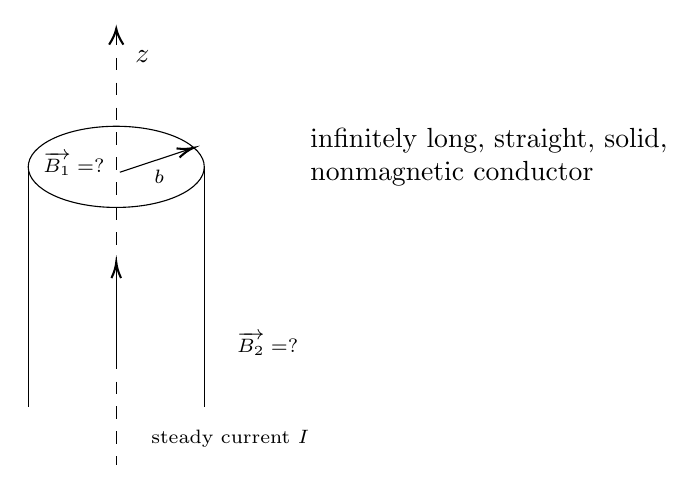
\begin{tikzpicture}[x=0.75pt,y=0.75pt,yscale=-1,xscale=1]
%uncomment if require: \path (0,300); %set diagram left start at 0, and has height of 300

%Straight Lines [id:da027460109812628142] 
\draw  [dash pattern={on 4.5pt off 4.5pt}]  (197.41,39.53) -- (197.41,193.82) -- (197.41,247.5) ;
\draw [shift={(197.41,37.53)}, rotate = 90] [color={rgb, 255:red, 0; green, 0; blue, 0 }  ][line width=0.75]    (7.65,-3.43) .. controls (4.86,-1.61) and (2.31,-0.47) .. (0,0) .. controls (2.31,0.47) and (4.86,1.61) .. (7.65,3.43)   ;
%Straight Lines [id:da07344532369289458] 
\draw    (199.16,106.67) -- (232.53,95.61) ;
\draw [shift={(234.43,94.98)}, rotate = 161.66] [color={rgb, 255:red, 0; green, 0; blue, 0 }  ][line width=0.75]    (7.65,-2.3) .. controls (4.86,-0.97) and (2.31,-0.21) .. (0,0) .. controls (2.31,0.21) and (4.86,0.98) .. (7.65,2.3)   ;
%Shape: Ellipse [id:dp020486684020196377] 
\draw   (155,104.09) .. controls (155,93.28) and (173.99,84.53) .. (197.41,84.53) .. controls (220.83,84.53) and (239.82,93.28) .. (239.82,104.09) .. controls (239.82,114.89) and (220.83,123.64) .. (197.41,123.64) .. controls (173.99,123.64) and (155,114.89) .. (155,104.09) -- cycle ;
%Straight Lines [id:da8393451238144485] 
\draw    (155,104.09) -- (155,220) ;
%Straight Lines [id:da31764526793844794] 
\draw    (239.82,104.09) -- (239.82,220) ;
%Straight Lines [id:da49253009541535164] 
\draw    (197.41,200) -- (197.41,152) ;
\draw [shift={(197.41,150)}, rotate = 90] [color={rgb, 255:red, 0; green, 0; blue, 0 }  ][line width=0.75]    (7.65,-2.3) .. controls (4.86,-0.97) and (2.31,-0.21) .. (0,0) .. controls (2.31,0.21) and (4.86,0.98) .. (7.65,2.3)   ;

% Text Node
\draw (205.33,46.73) node [anchor=north west][inner sep=0.75pt]    {$z$};
% Text Node
\draw (214.57,104.33) node [anchor=north west][inner sep=0.75pt]  [font=\scriptsize]  {$b$};
% Text Node
\draw (161.04,95.73) node [anchor=north west][inner sep=0.75pt]  [font=\scriptsize]  {$\overrightarrow{B_{1}} =?$};
% Text Node
\draw (254.38,182.4) node [anchor=north west][inner sep=0.75pt]  [font=\scriptsize]  {$\overrightarrow{B_{2}} =?$};
% Text Node
\draw (213.04,229.43) node [anchor=north west][inner sep=0.75pt]  [font=\scriptsize]  {$\text{steady current} \ I$};
% Text Node
\draw (289.71,84.35) node [anchor=north west][inner sep=0.75pt]   [align=left] {infinitely long, straight, solid,\\nonmagnetic conductor};
\end{tikzpicture}
\end{center}

\textit{\textbf{Sol.}}
	(a) Inside \\
\begin{minipage}[t]{0.3\textwidth}
	\begin{align*}
		& \oint_c \vec B \cdot \text{d} \vec l = \mu_0 I \\
		& \vec {B_1} = \hat{a_\phi} B_{\phi} \\
		& \text{d} \vec l = \hat{a_\phi} r_1 \text{d} \phi \\
		& I_1 = \frac{\pi r_1^2}{\pi b^2} I
	\end{align*}
\end{minipage}
\vline
\begin{minipage}[t]{0.6\textwidth}
  \begin{align*}
		& \Rightarrow \oint_{c_1} \hat{a_\phi} B_{\phi_1} \cdot \hat{a_\phi} r_1 \text{d} \phi = \mu_0 \cdot \frac{\pi r_1^2}{\pi b^2} I \\
		& \Rightarrow \int_{0}^{2 \pi} B_{\phi_1} r_1 \text{d} \phi = \mu_0 \cdot \frac{r_1^2}{b^2} I \\
		& 2 \pi B_{\phi_1} r_1 = \mu_0 \cdot \frac{r_1^2}{b^2}I \\
		& B_{\phi_1} = \frac{\mu_0 I r_1}{2 \pi b^2} \\ 
		\therefore &\vec{B_1} = \hat{a_\phi} B_{\phi_1} = \hat{a_\phi} \frac{\mu_0 I r_1}{2 \pi b^2}, \quad r_1 \leq b
  \end{align*}
\end{minipage}

	(b) Outside \\
\begin{minipage}[t]{0.3\textwidth}
	\begin{align*}
		& \oint_c \vec B \cdot \text{d} \vec l = \mu_0 I \\
		& \vec {B_1} = \hat{a_\phi} B_{\phi} \\
		& \text{d} \vec l = \hat{a_\phi} r_1 \text{d} \phi \\
		& I_2 = I
	\end{align*}
\end{minipage}
\vline
\begin{minipage}[t]{0.6\textwidth}
  \begin{align*}
		& \Rightarrow \oint_{c_2} \hat{a_\phi} B_{\phi_2} \cdot \hat{a_\phi} r_2 \text{d} \phi = \mu_0 I \\
		& \Rightarrow \int_{0}^{2 \pi} B_{\phi_2} r_2 \text{d} \phi = \mu_0 I \\
		& 2 \pi B_{\phi_2}r_2 = \mu_0 I\\
		& B_{\phi_2} = \frac{\mu_0 I}{2 \pi r_2} \\ 
		\therefore &\vec{B_2} = \hat{a_\phi} B_{\phi_2} = \hat{a_\phi} \frac{\mu_0 I}{2 \pi r_2}, \quad r > b
  \end{align*}
\end{minipage}
\newpage

\section*{Vector magnetic potential}
\begin{align*}
	\left.
  \begin{aligned}
		& \therefore \nabla \cdot (\nabla \times \vec{A}) = 0 \\
		& \therefore \nabla \cdot \vec{B} = 0
  \end{aligned}
  \right\}
  \quad \vec{B} \equiv \nabla \times \vec{A}
\end{align*}

$\vec A$: Vector magnetic potential $\quad \text{Wb}/\text{m}$
\begin{align*}
	& \therefore \nabla \times \vec B = \nabla \times \nabla \times \vec A \\
	& \because \nabla \times \vec B = \mu_0 \vec J \\
	& \Rightarrow \nabla \times \nabla \times \vec A = \nabla(\nabla \cdot \vec A) - \nabla^2 \vec A \\
  & \therefore \nabla(\nabla \cdot \vec A) - \nabla^2 \vec A = \mu_0 \vec J
\end{align*}
Choose $\nabla \cdot \vec A = 0$ (Coulomb guage) (為了使上式最簡化故選等於零)

\end{document}
